\section{Analysis}\label{sec:analysis}

\subsection{Invariant mass of final state particles}
The datasets consist of multiple events consisting of three particles $h_1 h_2 h_3$ that have been grouped together to form a candidate for a final state
of the decay $B^\pm \rightarrow h_1^\pm h_2^+ h_3^-$, where this ordering does not reflect the charges in the datasets.
To determine the invariant mass of the final state particles in both datasets the relativistic energy-momentum relation
\begin{equation}
  m(h_1 h_2 h_3)^2 = E(h_1 h_2 h_3)^2 - \vec{p}(h_1 h_2 h_3)^2
\end{equation}
where, due to 4-vector conservation, $E$ is the sum of the energies of the final state particles and $\vec{p}$ is the sum of the 3-momenta of the
final state particles. The 3-momenta have been measured or simulated, depending on the dataset, and are therefore contained in the data.
The energies are determined by rearranging the energy-momentum relation to
\begin{equation}
  E(h_i) = \sqrt{m(h_i)^2 + \vec{p}(h_i)^2}
\end{equation}
and assuming all final state particles to be kaons with mass $m(h_i) = 493.677 \, \si{\mega\eV}$ \cite{pdg}. The resulting momentum- and energy-distribution 
is shown in \autoref{f1}. The resulting mass spectrum, shown in \autoref{f2}, has a clear peak around the B-meson mass of 
$m_{B^0} = 5279.66 \pm 0.12 \si{\mega\eV}$ \cite{pdg} and follows a gaussian distribution due to the effects of the detector resolution, which 
also follows a gaussian distribution. 


\begin{figure}[H]
    \centering
    \begin{subfigure}{0.49\textwidth}
      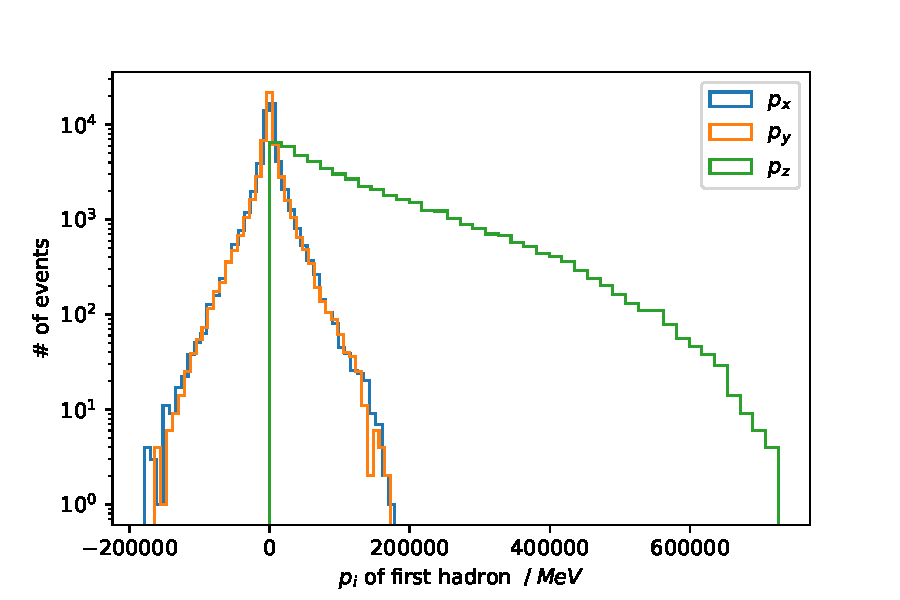
\includegraphics[width=\textwidth]{plots/momenta_H1_sim.pdf}
      \caption{Components of the 3-momentum of the first simulated hadron.}
      \label{fig:ProbPi}
    \end{subfigure}
    \begin{subfigure}{0.49\textwidth}
      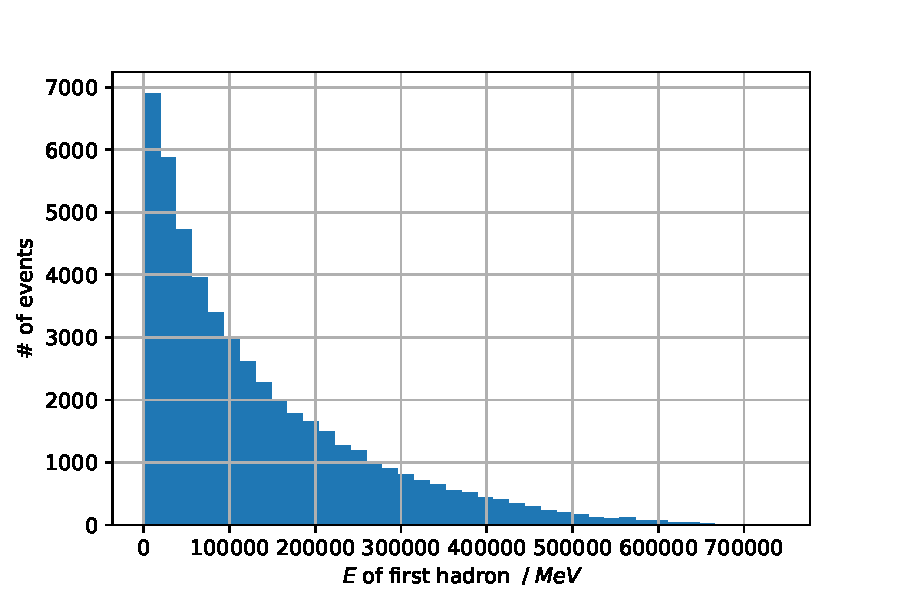
\includegraphics[width=\textwidth]{plots/energy_H1_sim.pdf}
      \caption{Energy of the first simulated hadron.}
      \label{fig:ProbK}
    \end{subfigure}
    \caption{Momentum components and energy of the first simulated hadron.}
    \label{f1}
    \end{figure}

\begin{figure}[H]
        \centering
        \begin{subfigure}{0.49\textwidth}
          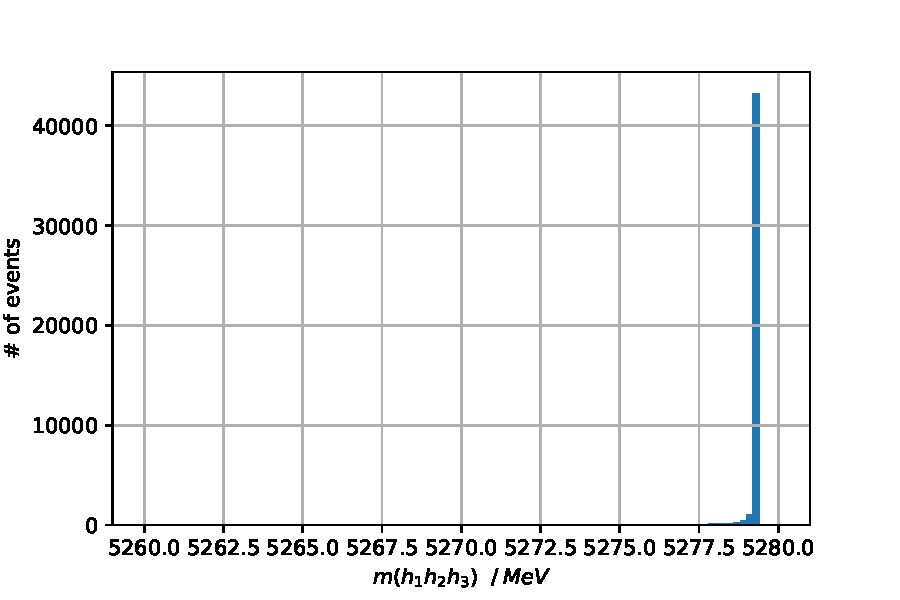
\includegraphics[width=\textwidth]{plots/mass_B_sim.pdf}
          \caption{Full spectrum of the invariant mass.}
          \label{fig:ProbPi}
        \end{subfigure}
        \begin{subfigure}{0.49\textwidth}
          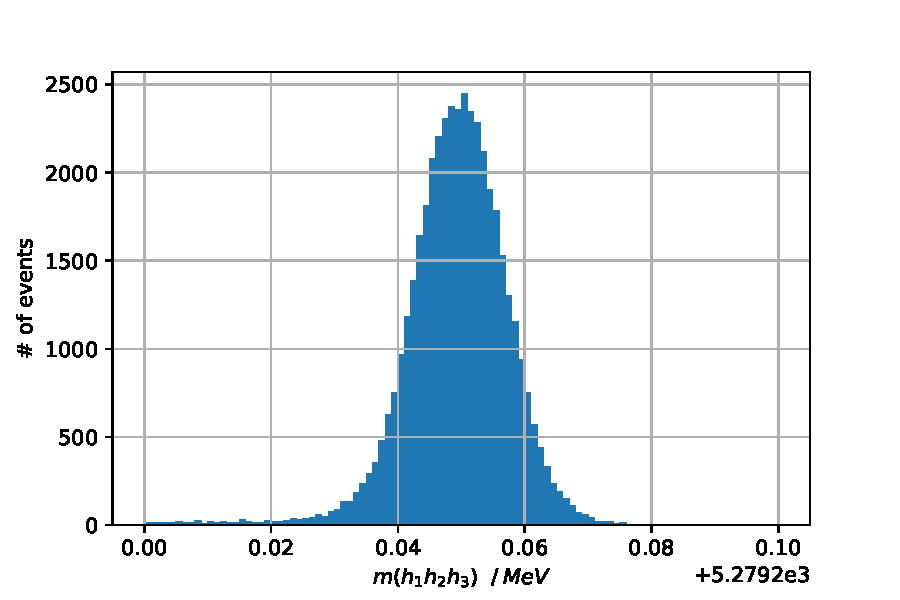
\includegraphics[width=\textwidth]{plots/masspeak_B_sim.pdf}
          \caption{Spectrum of the invariant mass restricted to $5279,2 \leq M \leq 5279,3$.}
          \label{fig:ProbK}
        \end{subfigure}
        \caption{Mass spectrum of the reconstructed B-mesons from simulated data.}
        \label{f2}
\end{figure}

To reduce the contribution of misidentified final state particles the probability that the
partcles are pions (\texttt{ProbPi}) and the probability that the particle is a kaon (\texttt{ProbK}) have been determined as shown
in \autoref{f3}. In addition the boolean
\texttt{IsMuon} encodes for each particle if it has been identified as a muon.
To reduce the background for every final state particle the cuts
\begin{itemize}
  \item $\texttt{probK} > 0.5$
  \item $\texttt{probPi} < 0.5$
  \item $\texttt{IsMuon} = false$
\end{itemize}
are applied. The resulting mass spectrum is shown in \autoref{f4}.
To further reduce the combinatorial background a cut on the invariant mass of the final state particles
\begin{itemize}
  \item $5200 \leq m \leq 5350$
\end{itemize}
is applied to the dataset with the real data. The resulting mass spectrum is shown in \autoref{f4b}.


\begin{figure}[H]
    \centering
    \begin{subfigure}{0.49\textwidth}
      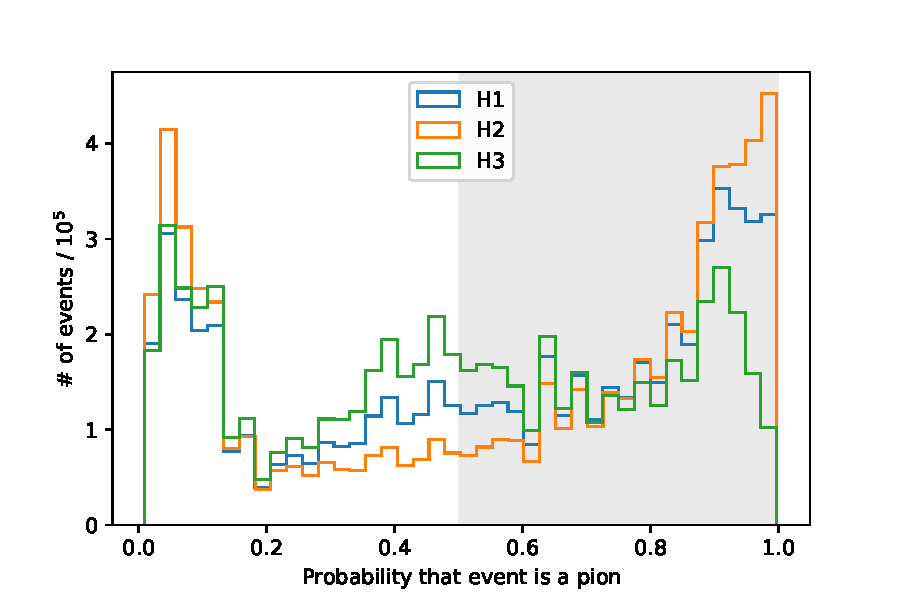
\includegraphics[width=\textwidth]{plots/ProbPi.pdf}
      \caption{Probability that the event is a pion.}
      \label{fig:ProbPi}
    \end{subfigure}
    \begin{subfigure}{0.49\textwidth}
      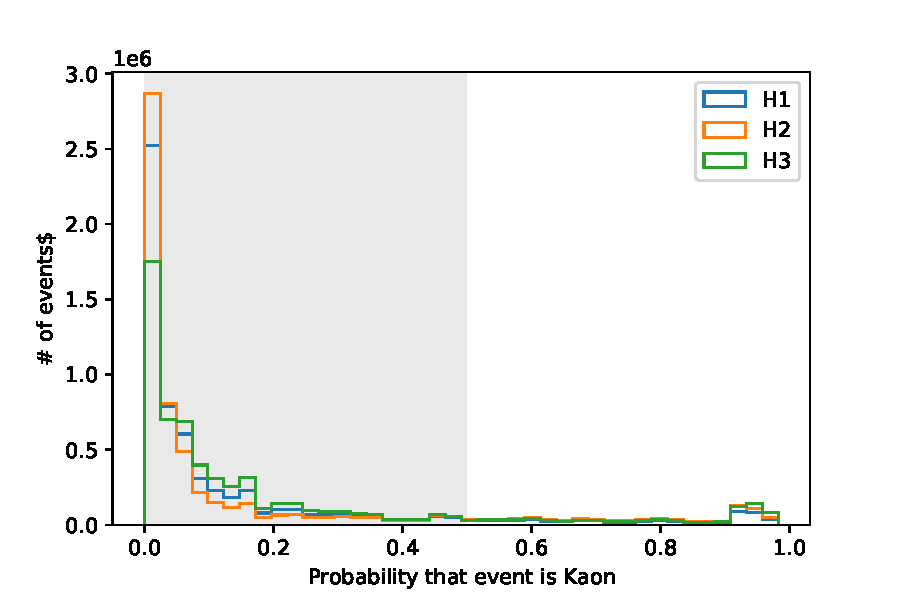
\includegraphics[width=\textwidth]{plots/ProbK.pdf}
      \caption{Probability that the event is a kaon.}
      \label{fig:ProbK}
    \end{subfigure}
    \caption{Probability spectrum that the measured hadron is either a pion or a kaon.
    The area with the grey background is removed by the cut on the pion- and kaon-probability.}
    \label{f3}
\end{figure}

\begin{figure}[H]
    \centering
    \begin{subfigure}{0.49\textwidth}
      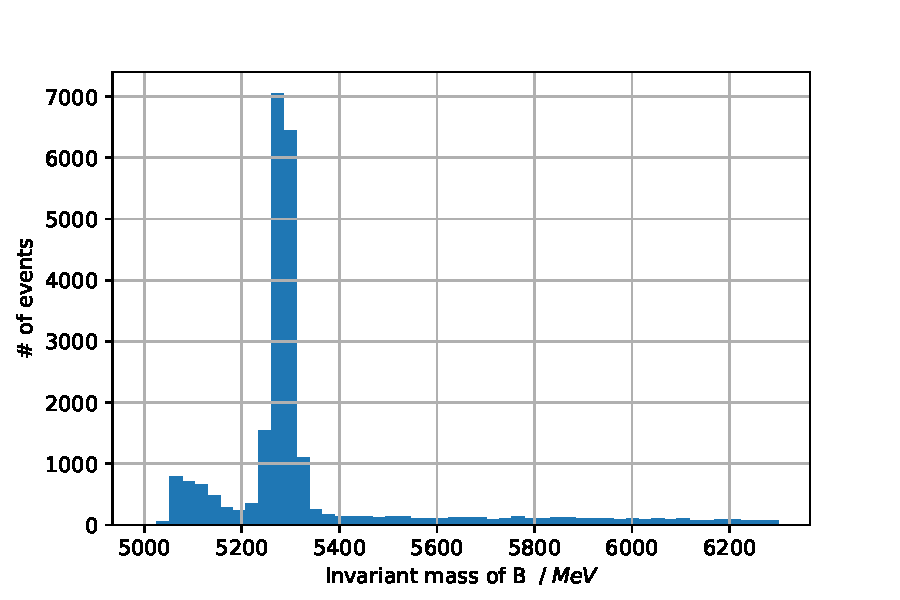
\includegraphics[width=\textwidth]{plots/mass_B.pdf}
      \caption{Full spectrum of the invariant mass.}
      \label{fig:ProbPi}
    \end{subfigure}
    \begin{subfigure}{0.49\textwidth}
      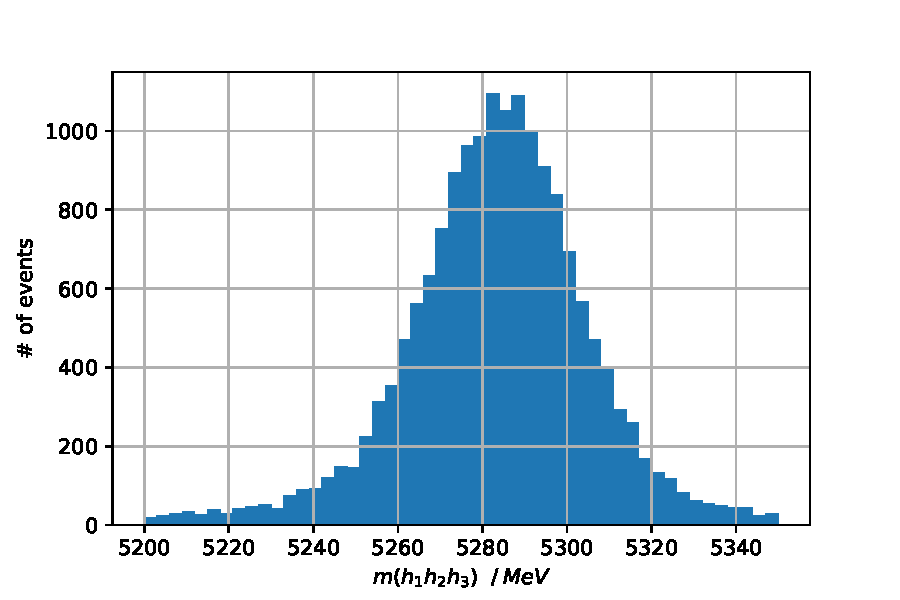
\includegraphics[width=\textwidth]{plots/masspeak_B.pdf}
      \caption{Spectrum of the invariant mass restricted to $5200 \leq m \leq 5350$.}
      \label{f4b}
    \end{subfigure}
    \caption{Mass spectrum of the B-mesons reconstructed from real data using the kaon mass hypothesis.}
    \label{f4}
\end{figure}

\subsection{The global \textit{CP}-asymmetry}
The number of $B^+$- and $B^-$-decays in the dataset with real data is determined by adding the charges of the final state
particles of each event. Utilizing this and \autoref{eq1} the global \textit{CP}-asymmetry is determined to be
\begin{equation}
  A_\textit{CP} = 0.050 \pm 0.008 (stat)
\end{equation}
with the uncertainty
\begin{equation}
  \sigma_A = \sqrt{\frac{1-A_\textit{CP}^2}{N^+ + N^-}}.
\end{equation}
and a significance of $6.504 \sigma$. This result does not take into account the expected production asymmetry of $\sim 1\%$.
The production asymmetry is modeled with an error in the measurement of $N^\pm$ of the form
\begin{equation}
  \Delta N^\pm (prod) = 0.01 \cdot N^\pm .
\end{equation}
Since the uncertainties in $N^+$ and $N^-$ are not independent the asymmetry is rewritten as
\begin{equation}
  A_\textit{CP} = \frac{N- 2 N^+}{N} = \frac{2 N^- - N}{N}
\end{equation}
to eliminate one of the variables. Both equations are used to determine the error of the asymmetry due to the production
asymmetry and the average
\begin{equation}
  \Delta A_\textit{CP} = 0.01
\end{equation}
is chosen to be the error.
Therefore the global \textit{CP}-asymmetry is found to be
\begin{equation}
  A_\textit{CP} = 0.05 \pm 0.01 (stat) \pm 0.01 (prod)
\end{equation}
with a significance of $3.98\sigma$.


%Using error propagation
%\begin{equation}
%  \Delta A_\textit{CP} (prod) = 0.02 \dot \frac{N^-}{N}
%\end{equation}
%can be drived and therefore
%\begin{equation}
%  A_\textit{CP} = 0.050 \pm 0.008 (stat) \pm 0.009 (prod)
%\end{equation}
%with a significance
%\begin{equation}
%  \text{significance} = \frac{A_\textit{CP}}{\sqrt{\sigma_A^2 + \Delta A(prod)^2}} = 4.106 \sigma .
%\end{equation}


%The production asymmetry modifies the uncertainty to
%\begin{equation}
%  \sigma_A^\prime = \sqrt{\sigma_A^2 + 0.01^2} = 0.013
%\end{equation}
%and reduces the significance of the global \textit{CP}-asymmetry to $3.978 \sigma$.

\subsection{The local \textit{CP}-asymmetry}
It is possible that the decay of $B^\pm$ proceeds through intermediate resonances. We expect resonances containing charm quarks
to be especially prominent. Since \textit{CP}-violation is much weaker in the charm-sector than in the b-sector we utilize
Dalitz plots to remove those intermediate resonances. Since the measured decays are of the form $B^\pm \rightarrow h_1^\mp h_2^\pm h_3^\pm$,
where $h$ is the measured final state particle, possible intermediate resonances are
\begin{align*}
  R_1^0 &\rightarrow h_1^\mp h_2^\pm \\
  R_2^0 &\rightarrow h_1^\mp h_3^\pm \\
  R_3^{\pm \pm} &\rightarrow h_2^\pm h_3^\pm .
\end{align*}
Since all relevant resonances are mesons, which can not have a charge of $\pm 2$, $R_3^{\pm \pm}$ is not investigated as an intermediate resonance.
The Dalitz plot generated from simulated and real data is shown in \autoref{f5}.
While the Dalitz plot from simulated data shows a homogeneus distribution over a given phasespace, the Dalitz plot from real data has three visible
resonances.

\begin{figure}[H]
  \centering
  \begin{subfigure}{0.49\textwidth}
    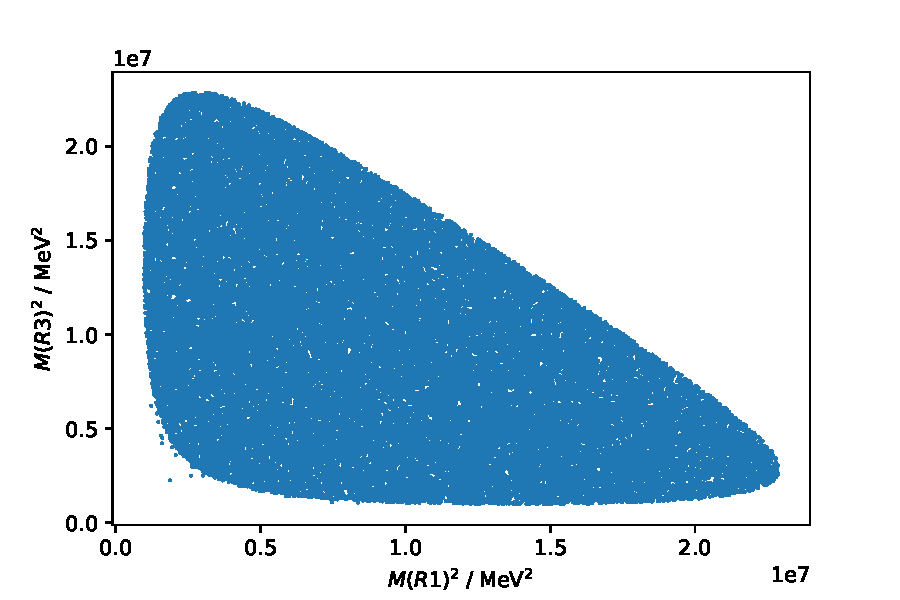
\includegraphics[width=\textwidth]{plots/Dalitz_sim_scatter.pdf}
    \caption{Scatterplot of the simulated data.}
    \label{fig:ProbPi}
  \end{subfigure}
  \begin{subfigure}{0.49\textwidth}
    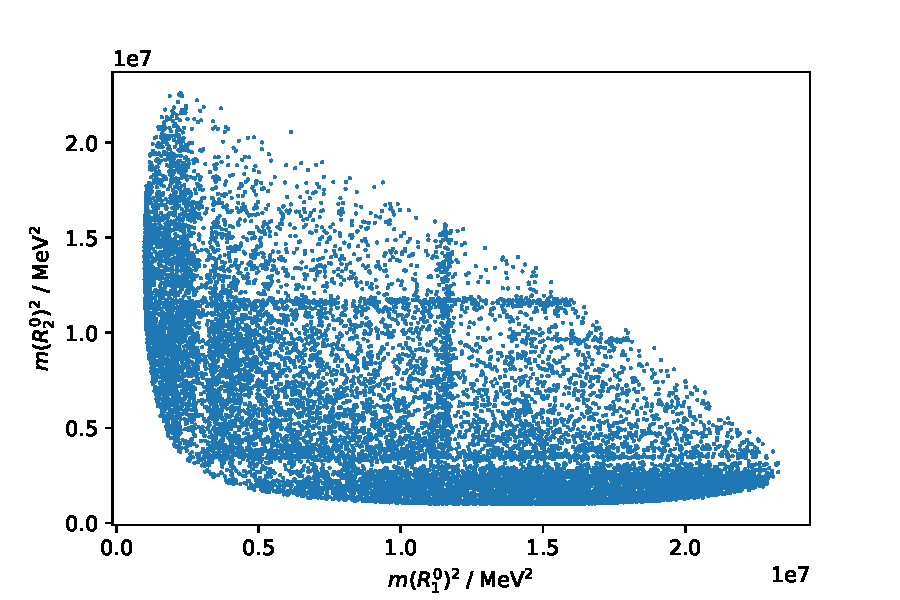
\includegraphics[width=\textwidth]{plots/Dalitz_scatter.pdf}
    \caption{Scatterplot of the real data.}
    \label{fig:ProbPi}
  \end{subfigure}
  \caption{Dalitz plots created from simulated and real data as a scatterplot}
  \label{f5}
\end{figure}

To reduce the phasespace and therefore to make the resonances more visible the symmetry of $h_2^0 \leftrightarrow h_3^0$ is
exploited. This is done by introducing an ordering of the intermediate states according to their invariant masses for each event
\begin{align*}
  R_\text{max} &= \{R_i^0 | m(R_i^0) > m(R_j^0) , \, i,\,j \in {1, \, 2}\} \\
  R_\text{min} &= \{R_i^0 | m(R_i^0) < m(R_j^0) , \, i,\,j \in {1, \, 2}\}
\end{align*}
and creating a Dalitz plot with the new intermediate states $R_\text{min}$ and $R_\text{max}$.
The resulting plot is shown in \autoref{f6a}. The resonances are identified as $D^0$, $\chi_{c0}(1P)$ and $J/Psi(1S)$, as
shown in \autoref{f6b}, and removed with the cuts
\begin{itemize}
  \item $m(D^0) - 50 \, \si{\mega\eV} > M(R_{\text{min/max}})$ or $m(D^0) + 50 \, \si{\mega\eV} < M(R_{\text{min/max}})$
  \item $m(\chi_{c0}(1P)) - 50 \, \si{\mega\eV} > M(R_{\text{min/max}})$ or $m(\chi_{c0}(1P)) + 50 \, \si{\mega\eV} < M(R_{\text{min/max}})$
  \item $m(J/Psi(1S)) - 50 \, \si{\mega\eV} > M(R_{\text{min/max}})$ or $m(J/Psi(1S)) + 50 \, \si{\mega\eV} < M(R_{\text{min/max}})$
\end{itemize}
where $m(D^0) = 1864.84 \, \si{\mega\eV}$, $m(\chi_{c0}(1P)) = 3414.71 \, \si{\mega\eV}$ and $m(J/Psi(1S)) = 3096.9  \, \si{\mega\eV}$ \cite{pdg}
as shown in \autoref{f6c}.
After all cuts are applied the global \textit{CP}-asymmetry is determined to be
\begin{equation}
  A_\textit{CP} = 0.05  \pm  0.01 \pm 0.01
\end{equation}
with a significance to the Standard Model of $3.62 \sigma$.

\begin{figure}[H]
  \centering
  \begin{subfigure}{0.49\textwidth}
    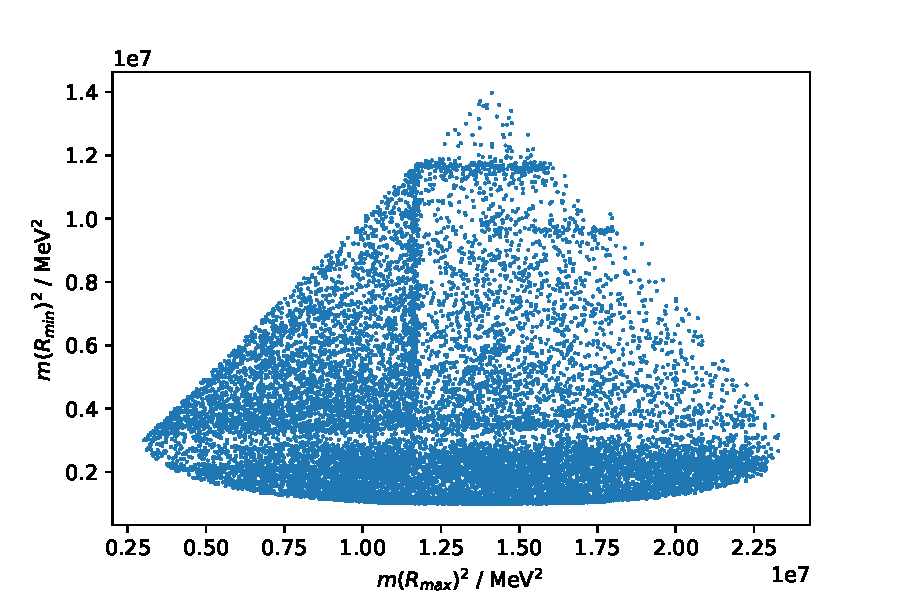
\includegraphics[width=\textwidth]{plots/Dalitz_sorted_scatter.pdf}
    \caption{Sorted Dalitz plot.}
    \label{f6a}
  \end{subfigure}
  \begin{subfigure}{0.49\textwidth}
    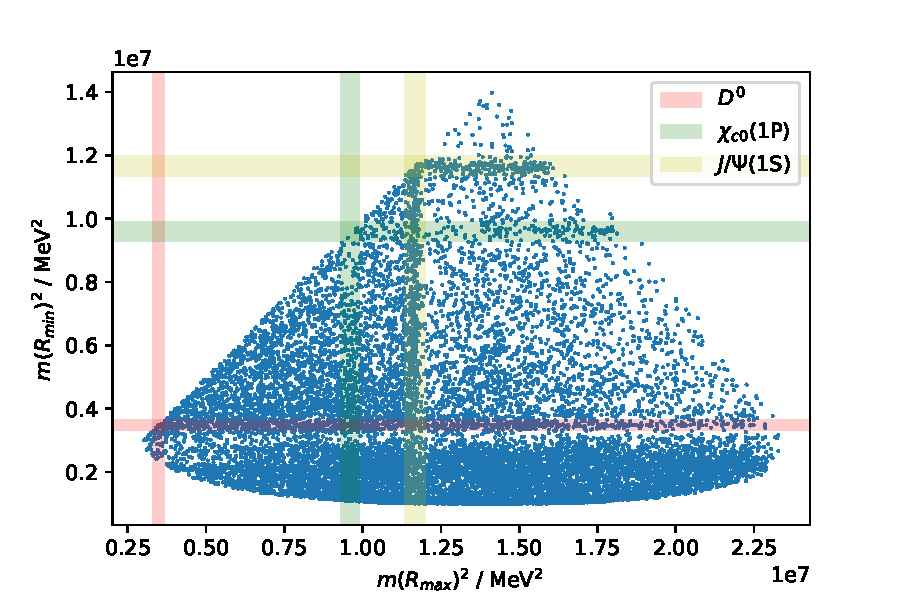
\includegraphics[width=\textwidth]{plots/Dalitz_sorted_scatter_band.pdf}
    \caption{Sorted Dalitz plot with events identified with resonance and removed by cuts marked by colored bands.}
    \label{f6b}
  \end{subfigure}
  \begin{subfigure}{0.49\textwidth}
    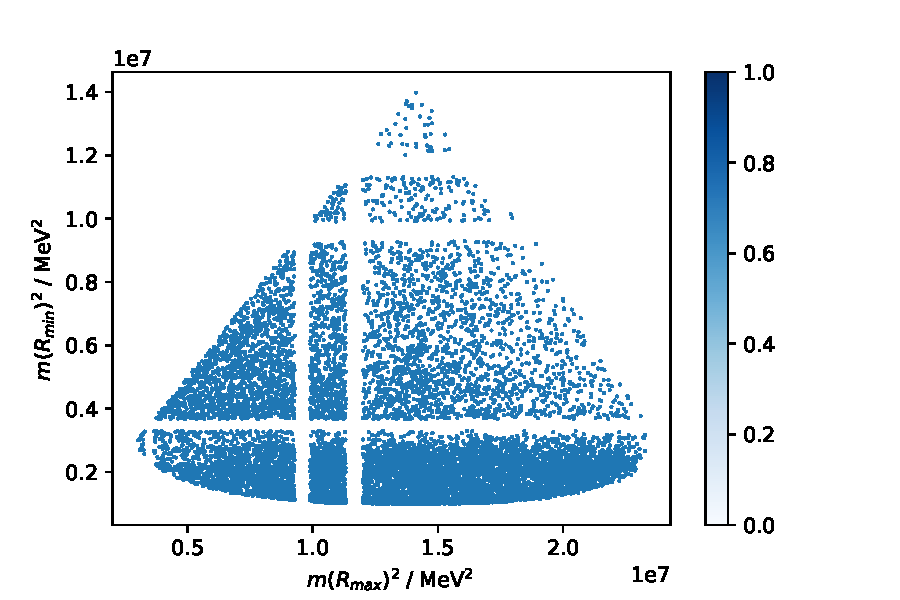
\includegraphics[width=\textwidth]{plots/Dalitz_sorted_scatter_cut.pdf}
    \caption{Sorted Dalitz plot after resonance cuts.}
    \label{f6c}
  \end{subfigure}
  \caption{The sorted Dalitz plots created from the real data before and after the application of the cuts for the removal of the resonances.}
  \label{f6}
\end{figure}

The new dataset is split into $6 \times 6$ bins and the number of $B^+$- and $B^-$-candidates is determined for each bin as shown in
\autoref{f7a} and \ref{f7b}. With this the local \textit{CP}-asymmetry is calculated for each bin as shown in \autoref{f7c}.
The significance of the \textit{CP}-asymmetry with the correction for the production asymmetry is shown in \autoref{f7d}.

\begin{figure}[H]
  \centering
  \begin{subfigure}{0.49\textwidth}
    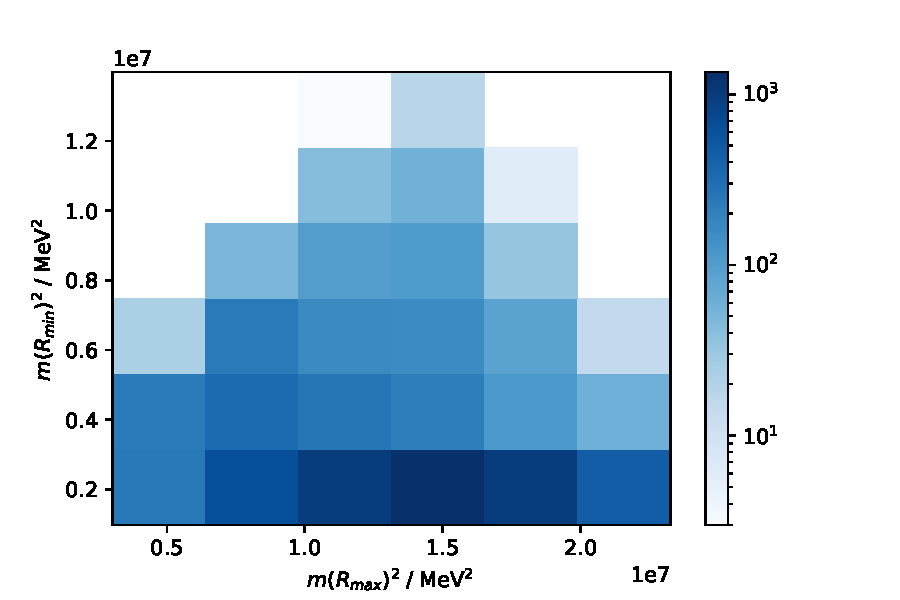
\includegraphics[width=\textwidth]{plots/Dalitz_sorted_bin_cut_bp.pdf}
    \caption{Binned histogram of the sorted Dalitz plot for the $B^+$-candidates.}
    \label{f7a}
  \end{subfigure}
  \begin{subfigure}{0.49\textwidth}
    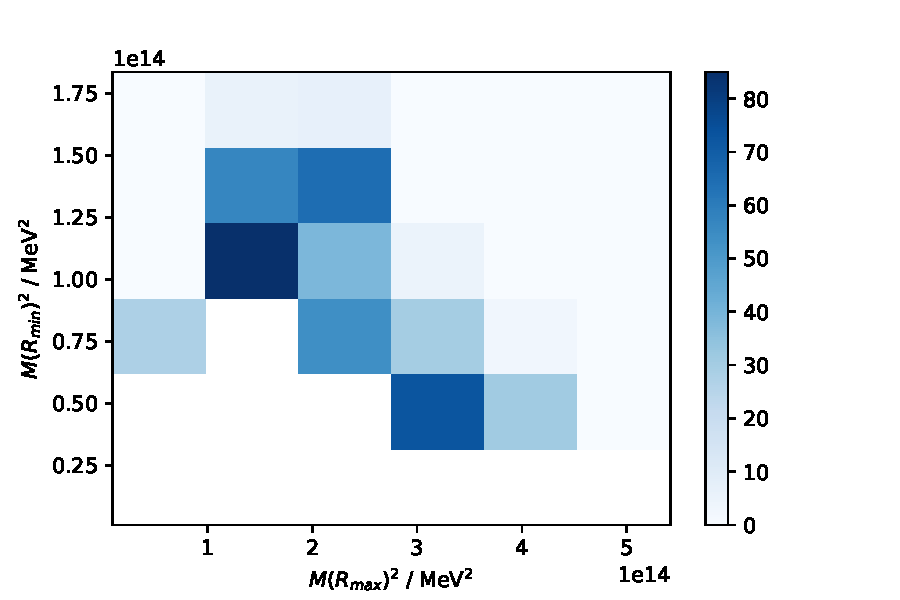
\includegraphics[width=\textwidth]{plots/Dalitz_sorted_bin_cut_bm.pdf}
    \caption{Binned histogram of the sorted Dalitz plot for the $B^-$-candidates.}
    \label{f7b}
  \end{subfigure}
  \begin{subfigure}{0.49\textwidth}
    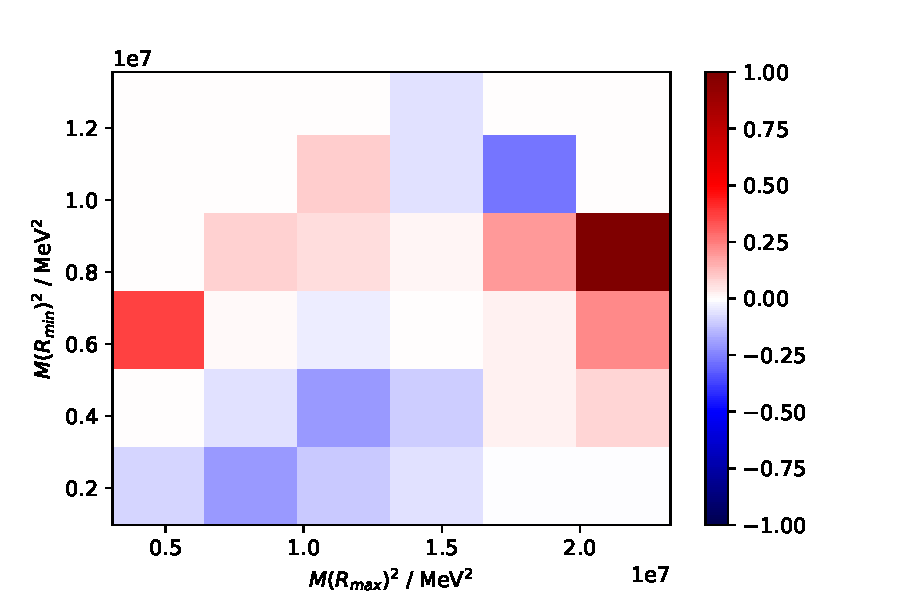
\includegraphics[width=\textwidth]{plots/Dalitz_sorted_Asym.pdf}
    \caption{The asymmetry calculated in each bin of the binned and sorted Dalitz plot.}
    \label{f7c}
  \end{subfigure}
  \begin{subfigure}{0.49\textwidth}
    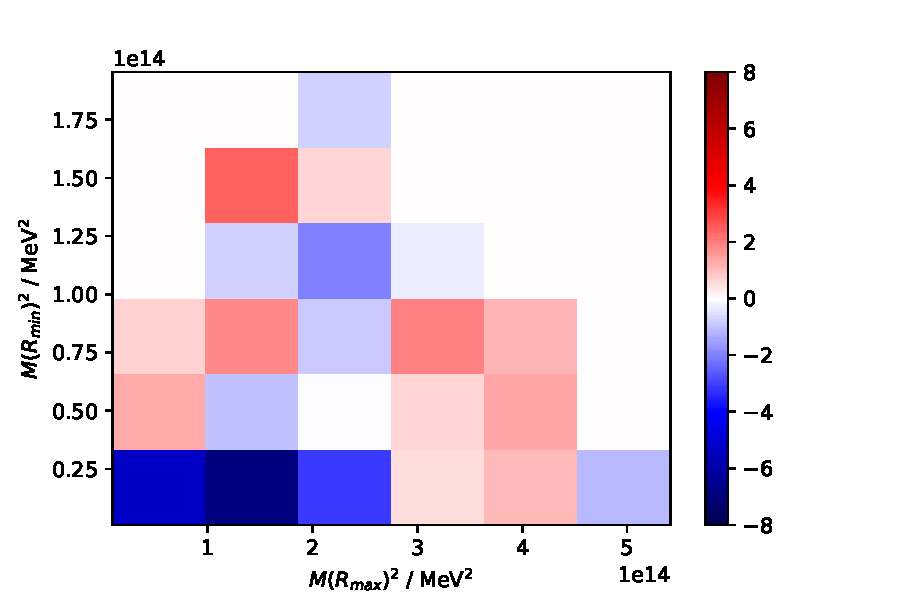
\includegraphics[width=\textwidth]{plots/Dalitz_sorted_bin_cut_sig.pdf}
    \caption{The significance calculated in each bin of the binned and sorted Dalitz plot.
    The area investigated for local \textit{CP}-asymmetry is enclosed by the yellow line.}
    \label{f7d}
  \end{subfigure}
  \caption{The binned sorted Dalitz plots determined for the $B^+$- and $B^-$-candidates and the significance and asymmetry calculated in each bin after the application
  of all cuts.}
  \label{f7}
\end{figure}

The largest significance in a bin where both decays have been reconstructed is observed in the bin
\begin{align*}
  0.64 \cdot 10^{7} \, \si{\mega\eV\squared} &\lesssim M(R_\text{max})^2 \lesssim 0.98\cdot 10^{7} \, \si{\mega\eV\squared} \\
  0.10 \cdot 10^{7} \, \si{\mega\eV\squared} &\lesssim M(R_\text{min})^2 \lesssim 0.31 \cdot 10^{7} \, \si{\mega\eV\squared}
\end{align*}
where the \textit{CP}-asymmetry is
\begin{equation}
  A_\textit{CP} = -0.20 \pm 0.03(stat)  \pm 0.01(prod)
\end{equation}
with a significance of $6.53 \sigma$. \\
The local \textit{CP}-asymmetry in the area enclosed by the yellow line in \autoref{f7d} is found to be
\begin{equation}
  A_\textit{CP} = -0.15  \pm 0.01  (stat)  \pm 0.01(prod)
\end{equation}
with a significance of $8.73 \sigma$. The mass spectrum for the $B^+$- and $B^-$-candidates in the area is shown in \autoref{f8}.

\begin{figure}[H]
  \centering
    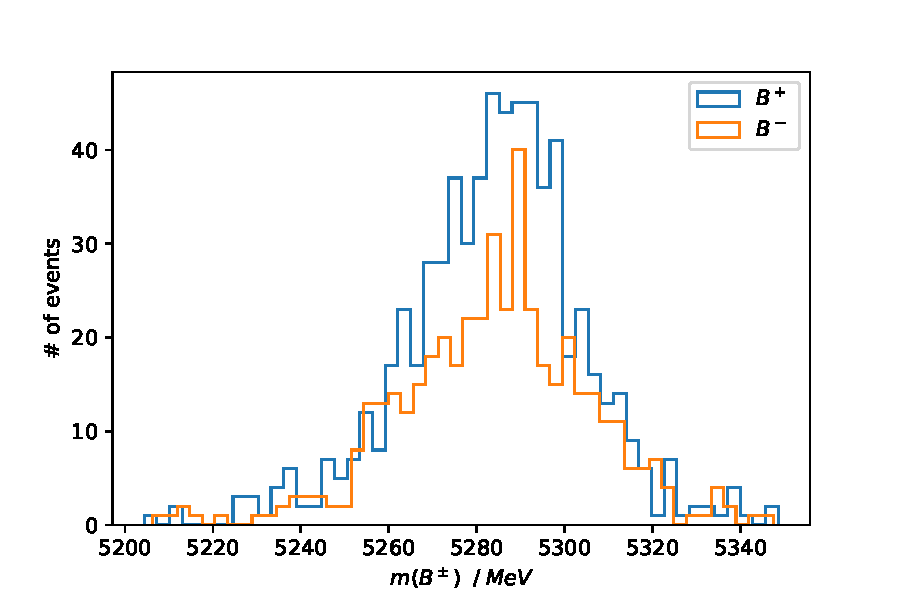
\includegraphics[width=\textwidth]{plots/num_b.pdf}
  \caption{The mass spectrum of the reconstructed $B^+$- and $B^-$-candidates in the area investigated for local \textit{CP}-asymmetry marked in \autoref{f7d}.}
  %$0.64 \cdot 10^{7} \, \si{\mega\eV\squared} \lesssim M(R_\text{max})^2 \lesssim 0.98\cdot 10^{7} \, \si{\mega\eV\squared}$ and
  %$0.10 \cdot 10^{7} \, \si{\mega\eV\squared} \lesssim M(R_\text{min})^2 \lesssim 0.31 \cdot 10^{7} \, \si{\mega\eV\squared}$.}
  \label{f8}
\end{figure}
